\documentclass[a4paper,12pt,titlepage]{article}

% Packages
\usepackage{animate}
\usepackage{amsmath}
\usepackage{amssymb}
\usepackage{bibentry}
\usepackage{color}
\usepackage{dirtree}
\usepackage{float}
\usepackage{geometry}
\usepackage{graphicx}
\usepackage{hyphenat}
\usepackage{indentfirst}
\usepackage{listings}
\usepackage{ipsum}
\usepackage{titlesec}
\usepackage{url}
\usepackage{physics}
\usepackage{fontspec}
\usepackage{wrapfig}
\usepackage{subcaption}
\usepackage{float}
\usepackage[normalem]{ulem}
\usepackage[backend=biber, style=apa]{biblatex}
\usepackage[
colorlinks=true,
linkcolor=blue,
urlcolor=cyan,
citecolor=blue,
breaklinks=true,
]{hyperref} % For hyperlinks

\definecolor{dkgreen}{rgb}{0,0.6,0}
\definecolor{gray}{rgb}{0.5,0.5,0.5}
\definecolor{mauve}{rgb}{0.58,0,0.82}
\lstset{
	aboveskip=3mm,
	basicstyle=\ttfamily\small,
	belowskip=3mm,
	breakatwhitespace=true,
	breaklines=true,
	columns=flexible,
	commentstyle=\color{dkgreen},
	frame=none,
	keywordstyle=\color{blue},
	language=C++,
	numbers=none,
	numberstyle=\tiny\color{gray},
	showstringspaces=false,
	stringstyle=\color{mauve},
	tabsize=4
}
\addbibresource{references.bib}
\geometry{margin=1in}
\titleformat{\chapter}[display]
{\normalfont\huge\bfseries}{\chaptertitlename\ \thechapter}{20pt}{\Huge}
\titlespacing{\chapter}{0pt}{0pt}{0pt}
\sloppy

% Title and Author
\title{Computational Fluid Dynamics With a Paper Airplane}
\author{
  Tasada, Daniel\\
  \and
  Tse, Nathan\\
}
\date{\today}

% Title and abstract
\begin{document}
\maketitle
\begin{abstract}
	In this paper, we investigate the relationship between an airplane's shape
	and its performance. Our results show that \dots
\end{abstract}

% Table of Contents
\pagebreak
\section{Preface}
\ipsum[1]

\pagebreak

\tableofcontents
\pagebreak

\section{Nomenclature}
\textit{Acronyms:}
\[
	\begin{array}{ll}
		\text{CFD} & \text{Computational Fluid Dynamics} \\
		\text{ML} & \text{Machine Learning} \\
		\text{NEAT} & \text{NeuroEvolution of Augmenting Topologies} \\
		\text{BVH} & \text{Bounding Volume Hierarchy} \\
		\text{FCL} & \text{Flexible Collision Library} \\
		\text{AMR} & \text{Adaptive Mesh Refinement} \\
	\end{array}
\]

\textit{Variables:}
\[
	\begin{array}{ll}
		L & \text{Angular momentum of a given particle} \\
		I & \text{Inertia tensor of a given particle} \\
		\omega & \text{Angular velocity of a given particle} \\
		n & \text{Collision normal of a given particle} \\
		R_i & \text{Orientation of a given particle} \\
		\lambda & \text{Constant used in Lagrangian collision resolution} \\

		\\

		u & \text{Velocity} \\
		\rho & \text{Density} \\
		\nu & \text{Viscosity} \\
		\kappa & \text{Density diffusivity} \\
		f & \text{External forces} \\
		S & \text{Density source}

		\\
		
		\tau & \text{Shear stress} \\
		P & \text{Pressure} \\
	\end{array}
\]
\pagebreak

% Introduction
\section{Introduction}
This thesis covers the simulation of the aerodynamics of an airplane, using
our own Computational Fluid Dynamics model (CFD).

The goal is to simulate the airflow around an airplane's body. CFD is a
branch of fluid mechanics that uses numerical methods and algorithms to solve
and analyze problems that involve fluid flows. It is used in many fields,
including aerospace engineering, automotive engineering, and meteorology.

The application of CFD to an airplane is important because it allows testing
of a model's aerodynamic performance without building a physical model, or
have to set up a wind tunnel. The practical alternative is much more expensive
and time-consuming.

CFD is challenging in the sense that it requires a good understanding of fluid
dynamics, as well as a good understanding of the math involved. CFD is also
very expensive from a computational perspective, so code optimization is important.

The final aim is to determine how the shape of an airplane's body affects its
performance. The intention is to use machine learning to optimize the shape of the airplane's body to maximize
performance. Therefore the question we will try to answer in this paper is: \\

\textbf{What is the most optimal shape for an airplane to maximize its aerodynamic performance?} \\

The question will be divided into the following sub-questions: \\

\textbf{SQ1:} How does a basic a CFD model work? \\

Because we will be making our own CFD model, it is important that we understand how a CFD model works. 
Answering this question will give us a good idea of how we can create our own CFD model. \\

\textbf{SQ2:} How is a CFD model implemented? \\

Not only is understanding how a CFD model works important, but also how it is implemented. 
Part of the research done to answer this question will be by analyzing other existing CFD models.
After answering this question we will have created a basic CFD model. \\

\textbf{SQ3:} How do obstacles work in a CFD?\\

To answer our main question we will need to implement the way the airplane interacts with the fluid. 
That is why answering \textbf{SQ3} is an important part of our research. 
It will give us the possibilty to analyze how the airplane's shape affects it performance. \\

\textbf{SQ4:} How is the performance of an airplane calculated? \\

We want to be able to compare different airplane shapes to see which one has the best aerodynamic performance 
To be able to know how well an airplane is performing we need to how performance is defined
The answer to this question will give us that definition and also the information we need to compare the different airplane shapes.\\

\textbf{SQ5:} How can machine learning be used to optimize an airplane's shape? \\

A part of the research will require us to use machine learning. 
This is so that the we can optimize the shape of the airplane way faster and more efficiently than we could do by hand.
That is why the answer \textbf{SQ5} will in the end help us to find the answer to our main question. 

\pagebreak

\section{Preliminary Research}
In this paper we aim to create our own CFD model and use machine learning to research the aerodynamics of an airplane.
Before we start creating our own model, an understanding of how CFD works 
and the different types of models and methods that can be used is needed.
Most CFD models are based on the Navier-Stokes equations. Because the Navier-Stokes equations are very complex we will not be covering them in depth, 
but we will explain what they are and how they are used in CFD models.
This will be covered in section \ref{navierstokes}.
In section \ref{eulerianlagrangian} we will be looking at two different types of methods that are used to simulate fluid dynamics.
For the machine learning part, we will be using a genetic algorithm to optimize the shape of the airplane. 
What genetic algorithms are and how they work will be covered in section \ref{genalgsec}.

\subsection{Navier-Stokes equations} \label{navierstokes}
The base of almost all CFD models are the \href{https://en.wikipedia.org/wiki/Navier%E2%80%93Stokes_equations}{Navier-Stokes equations}.
These are partial differential equations that describe fluid flows. 
We will not go into too much detail about these equations, but the gist of it that these equations return the flow velocity of the fluid.
This flow velocity is a vector field that assigns a vector to every point in the fluid at a given time. 
Using this velocity field, the behavior of the fluid can be simulated.
(\cite{navierstokes})

\subsection{Eulerian vs Lagrangian} \label{eulerianlagrangian}
There are two main methods to simulate fluid dynamics: the Lagrangian method and the Eulerian method.

\paragraph{Lagrangian}\mbox{}

\begin{figure}[H]
	\centering
	\includegraphics[width=10cm]{resources/lagrangian.png}
	\caption{Lagrangian fluid simulation from (\cite{seblague})}
\end{figure}

The Langrangian method models the fluid as a particle collision system, where the air is represented by
particles that follow the flow velocity and interact with each other to emulate a fluid. 
This method is mostly useful when trying to analyze situations where single fluid particles play an important role.

\pagebreak
\textbf{Eulerian} \\

\begin{figure}[H]
	\centering
	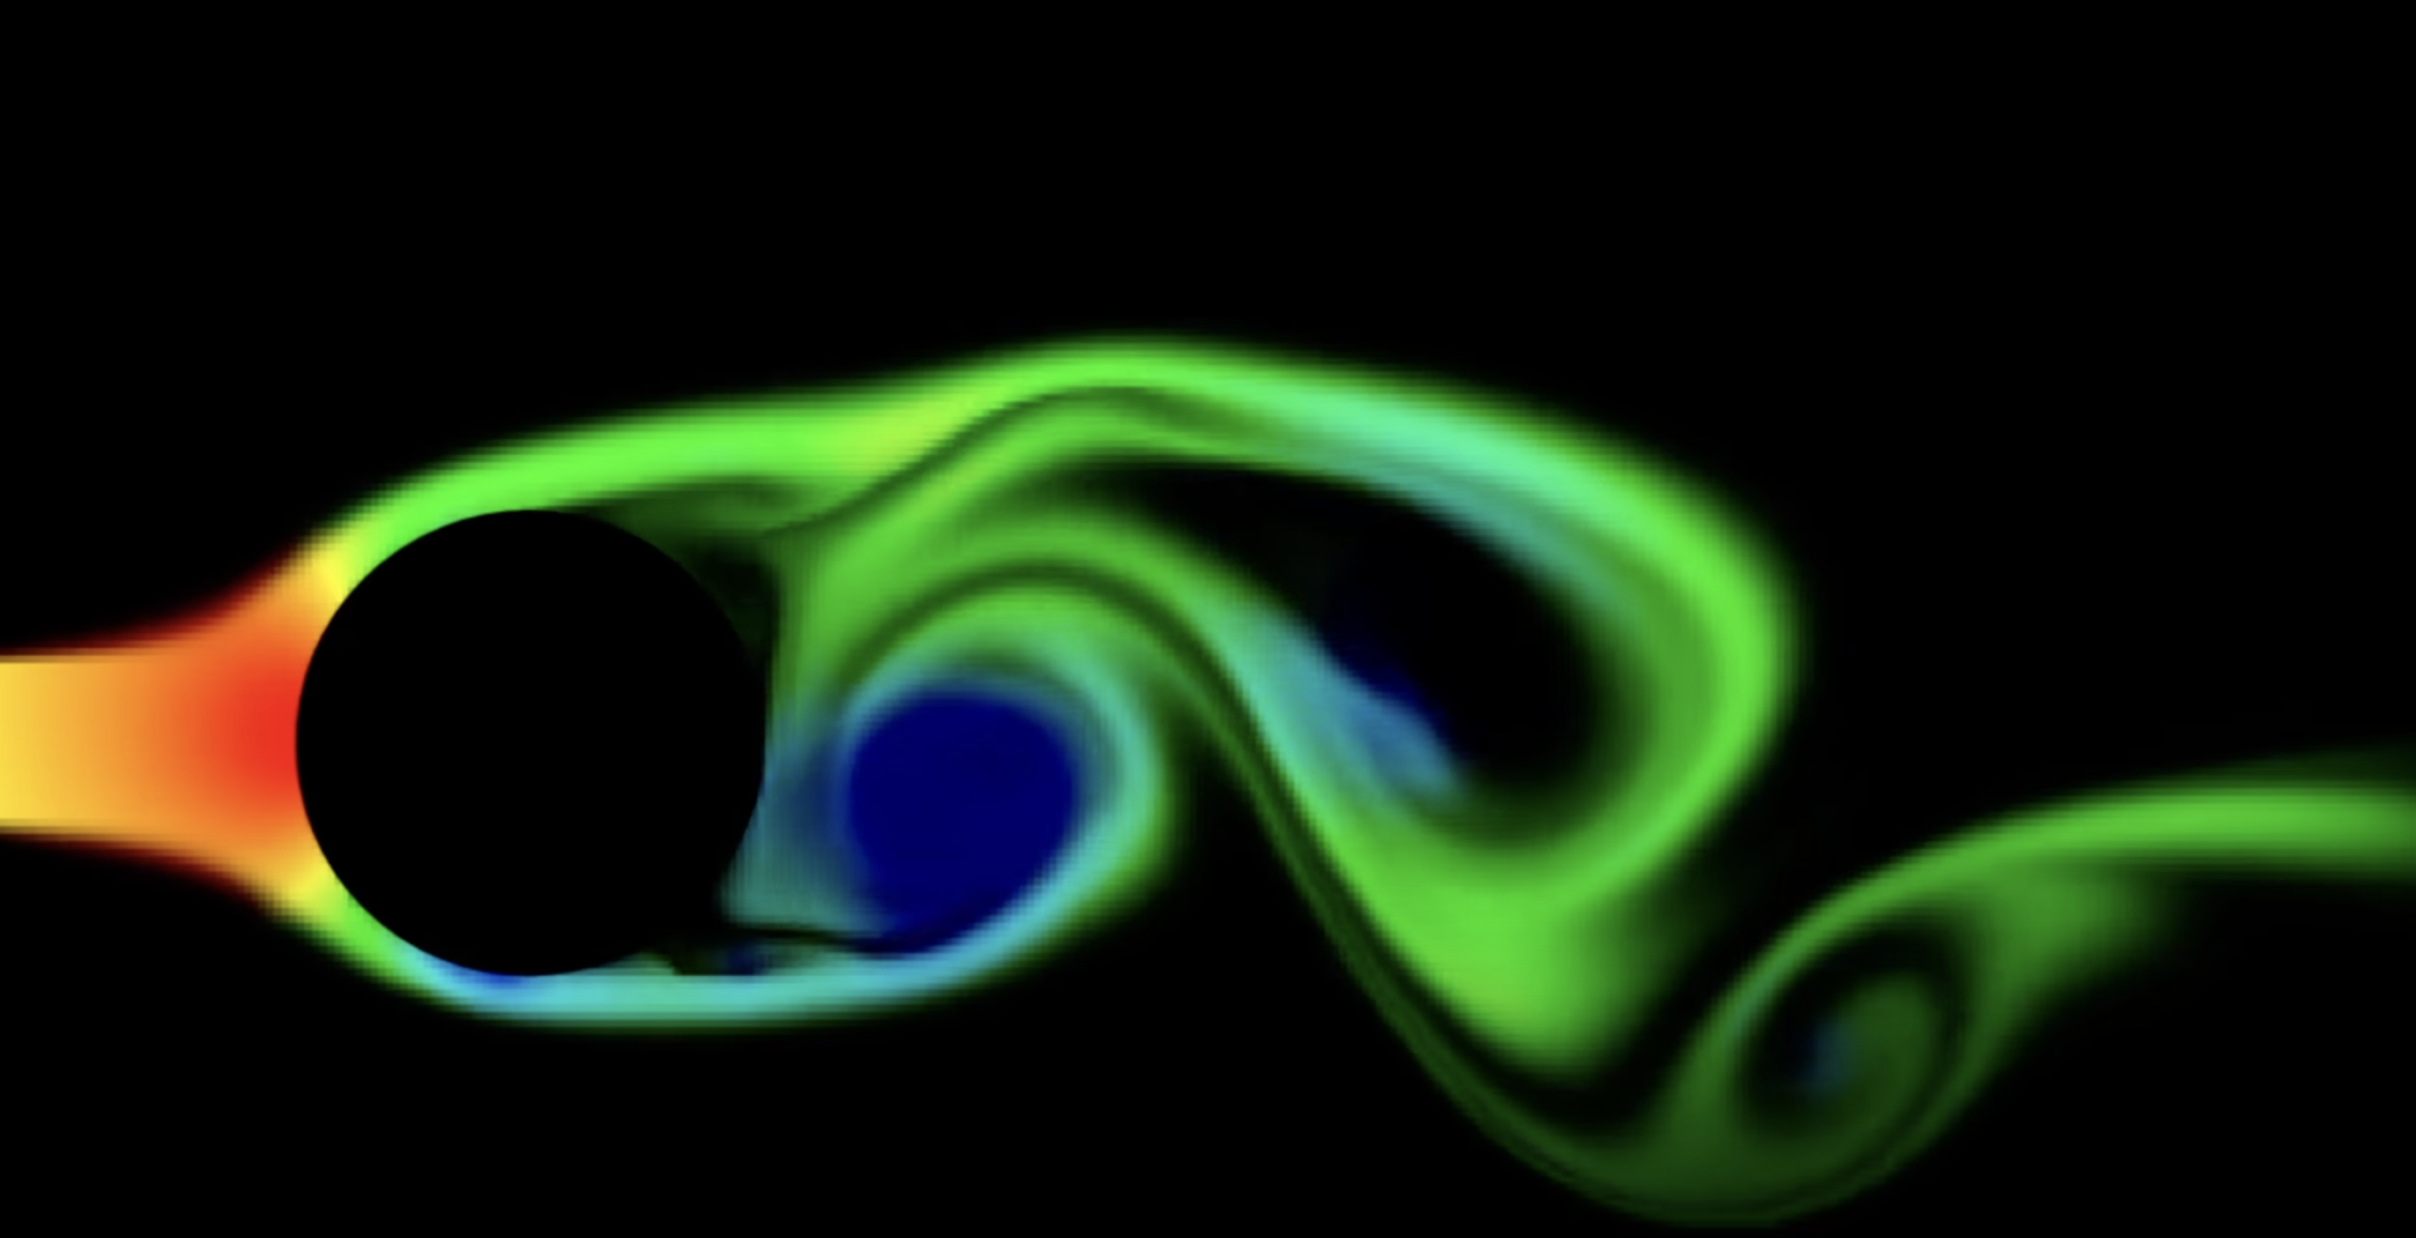
\includegraphics[width=10cm]{resources/eulerian.png}
	\caption{Eulerian fluid simulation from (\cite{tenminute})}
\end{figure}

The other method is the Eulerian method. This method models the fluid as a
cellular automata. The fluid is represented by a grid of cells, each of which
has its own properties and interacts with its neighbor cells, creating a continuous
field. This method is mostly used when trying to analyze the fluid as a whole.
It can provide information about the fluid's flow patterns, turbulence, and pressure distribution. 

\subsection{Genetic Algorithm} \label{genalgsec}
In machine learning, genetic algorithms are models that mimic the process of natural selection.
In a genetic algorithm a population of solutions to an optimization problem is evolved over time towards better solutions.
The evolution usually starts from a population of randomly generated solutions.
It is an iterative process, where the population in each iteration is called a generation.
A fitness function is used every generation to evaluate the fitness of each solution in the population.
Fitness is a measure of how well a solution fits the problem.
With that in mind an iteration will typically look like this:
\begin{enumerate}
	\item{The fitness of every solution in the population is evaluated.}
	\item{A percentage of the more fit solution are selected from the current population.}
	\item{Each selected solution is randomly modified.}
	\item {These fit solutions and the new mutated solutions are added to the new generation.}
	\item{The new generation of candidate solutions is then used in the next iteration of the algorithm.}
\end{enumerate}
(\cite{genalg})

% Execution
\pagebreak
\section{First Prototype: Lagrangian Fluid Simulation}
We first tried to implement a Lagrangian fluid simulation.
Our implementation is based on \hyperlink{http://www.hakenberg.de/diffgeo/collision_resolution.htm}{Rigid Body Collision Resolution}
(\cite{hakenberg}). We used this paper as a guide for all the math involved.

The math relies on the momentum, inertia, and velocity of the particles to
calculate the collision normal and point of contact. The collision normal is
the direction in which the particles are moving away from each other, and the
point of contact is the point at which the particles collide.

The following variables are necessary to perform the calculations:
\[
\begin{array}{ll}
	\text{Angular momentum $L$ } (kg\cdot m^2/s): & L = mvr; \\
	\text{Inertia tensor $I$ } (kg\cdot m^2): & I = \frac{L}{\omega}; \\
    \text{Angular velocity $\omega$ } (rad/s): & \omega = \frac{\Delta \theta}{\Delta t}; \\

	\\

	\text{Collision normal} (n \in \mathbb{R}^3) \text{ in world coordinates away from body}; \\
	\text{Point of contact } (r_i \in \mathbb{R}^3) \text{ in world coordinates with respect to $p_i$}; \\
	\text{Orientation } (R_i \in SO(3)) \text{ transforming from object to world coordinates}; \\
\end{array}
\]

Where $i$ represents one of two particles in a given collision:
\[
\begin{array}{ll}
	\text{Velocity after collision} & \tilde{v}_i, \\ 
	\text{Angular velocity after collision} & \tilde{\omega}_i, \\
	\text{Constant} & \lambda, \\
\end{array}
\]

The following formulas represent the relation between particles:
\[
\begin{array}{cc}
	\tilde{v}_1 = v_1 - \frac{\lambda}{m_1} n; \\ 
	\tilde{v}_2 = v_2 + \frac{\lambda}{m_2} n; \\
	\tilde{\omega}_1 = \omega_1 - \Delta q_1; \\
	\tilde{\omega}_2 = \omega_2 + \Delta q_2; \\

	\text{where } q_i := I_i^{-1} \cdot R_i^{-1} \cdot (r_i\times n), \\
	\text{and } \lambda = 2 \frac{n v_1 - n v_2 + \omega_1 I_1 q_1 - \omega_2 I_2 q_2}
	{(\frac{1}{m_1} + \frac{1}{m_2})n^2 + q_1 I_1 q_1 + q_2 I_2} \\
\end{array}
\]

This was implemented using Go and raylib, and the code is available at
\href{www.github.com/dtasada/paper}{github.com/dtasada/paper} at the \lstinline[breaklines]{lagrangian-go} branch.

When dealing with a lot of particles, the simulation stops performing as well,
because the number of calculations and iterations of the formulas listed above
has a time complexity of $O(n^2)$, where $n$ is the number of particles. This is
because every particle handles collisions with every other particle every
single frame. This can be elegantly mitigated by implementing a three-dimensional
grid system, where every particle is assigned to a cell in the grid. This way,
particles only need to check for collisions with other particles in the same cell
or in any of its 26 neighboring cells, assuming that the particles are evenly
distributed within the container, each particle only needs to handle collisions
with particles in its own cell, and its 26 neighboring cells. This reduces the
time complexity to $O(n)$.

The simulation was unstable at higher densities, where particles would phase
into each other instead of cleanly bouncing. The bug is likely quite simple to
fix, but we got distracted by the Eulerian method. Despite the optimizations we
made, Lagrangian simulation is still quite computationally expensive, and Go
wasn't doing it any favors, because it's not a very memory efficient language.
In the end it was put aside, and the Lagrangian implementation was never completed.

\pagebreak
\section{Execution: Eulerian Fluid Simulation}

\noindent
\begin{minipage}[t]{0.65\textwidth}
	Our next attempt was to try and implement a Eulerian fluid simulation.
	Our fluid simulation involves a three-dimensional grid of cells, each of which
	have velocity and density fields. The density fields are purely for the purpose
	of visualization. In the CFD frontend, we render translucent colored cubes in
	each cell according to its density field. These translucent cubes represent
	dye getting dropped into the container. When we are talking about `density',
	you can image it as the density of dye in the fluid. Each frame, the cells
	interact with each other according to the \href{https://en.wikipedia.org/wiki/Navier%E2%80%93Stokes_equations}{Navier-Stokes equations}.
	\end{minipage}\hfill
	\begin{minipage}[t]{0.3\textwidth}
		\vspace{4pt}
		\centering\raisebox{\dimexpr \topskip-\height}{%
		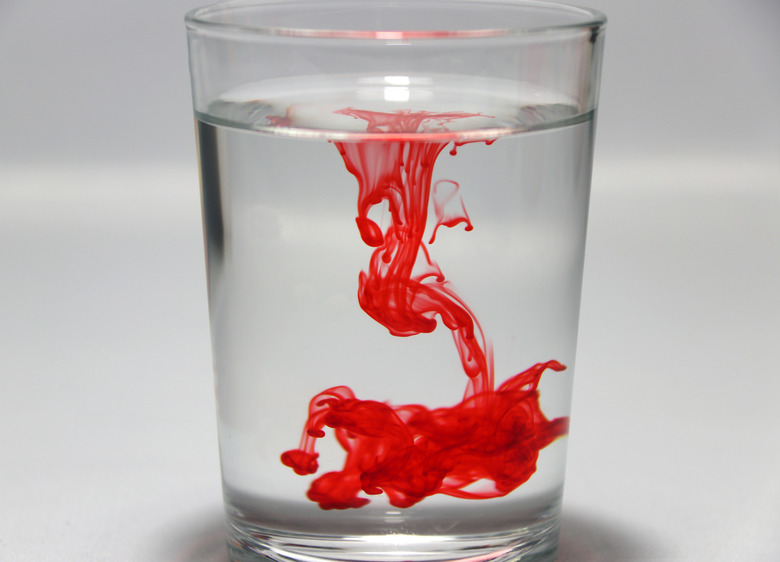
\includegraphics[width=\textwidth]{resources/dye.jpg}}
		\captionof{figure}{Dye diffusing in water}
	\end{minipage}

The specific math involved in the base equations for the fluid simulation is
quite complex, and we couldn't have derived it on our own, so we used
Mike Ash's implementation \href{www.mikeash.com/pyblog/fluid-simulation-for-dummies.html}{\citefield{mikeash}{title}} (\cite{mikeash})
as the bedrock of our program. Mike Ash's code is in turn based on Jos Stam's
brilliant work on \href{www.dgp.toronto.edu/public_user/stam/reality/Research/pdf/GDC03.pdf}{\citefield{josstam}{title}} (\cite{josstam}).
This math will be explained in section \ref{math}. 
How we implemented this math into the density solver of the fluid simulation is explained in section \ref{density}.
The way it is implemented in the velocity solver is explained in section \ref{velocity}.
We will explain the concepts in 2D, so it is easier to visualize and understand.
Lastly, section \ref{implementation} explains how to implement the fluid simulation,
which includes the code's structure and how we implemented the collision detection.

% Math
\subsection{The Math} \label{math}
In Eulerian fluid dynamics we represent fluids with a velocity vector field. This means we assign a velocity vector to every point in space.
The Navier-Stokes equations show us how these velocity vectors evolve over time with an infinitesimal timestep.
\[
	\begin{array}{ll}
		\text{velocity equation: } & \pdv{u}{t} = -(u \cdot \nabla)u + \nu\nabla^2 + f \\
		\\
		\text{density equation: } & \pdv{\rho}{t} = -(u \cdot \nabla)\rho + k\nabla^2\rho + S
	\end{array}
\]
The first equation returns the change in velocity in a vector notation. 
Unlike in Lagrangian fluid simulation, in Eulerian fluid simulation the fluid is not represented by individual particles. 
That's why fluid density is used instead, which tells us the amount of particles present in a point in space. 
The second equation shows us the change in density. 
Despite that it isn't needed to fully understand these equations to understand
the math behind the simulation, it should be noted that the two equations above look
a lot like each other, as this was helpful in developing the simulation. (\cite{josstam})

\begin{figure}[H]
	\centering
	\begin{subfigure}[t]{0.45\textwidth}
		\centering
		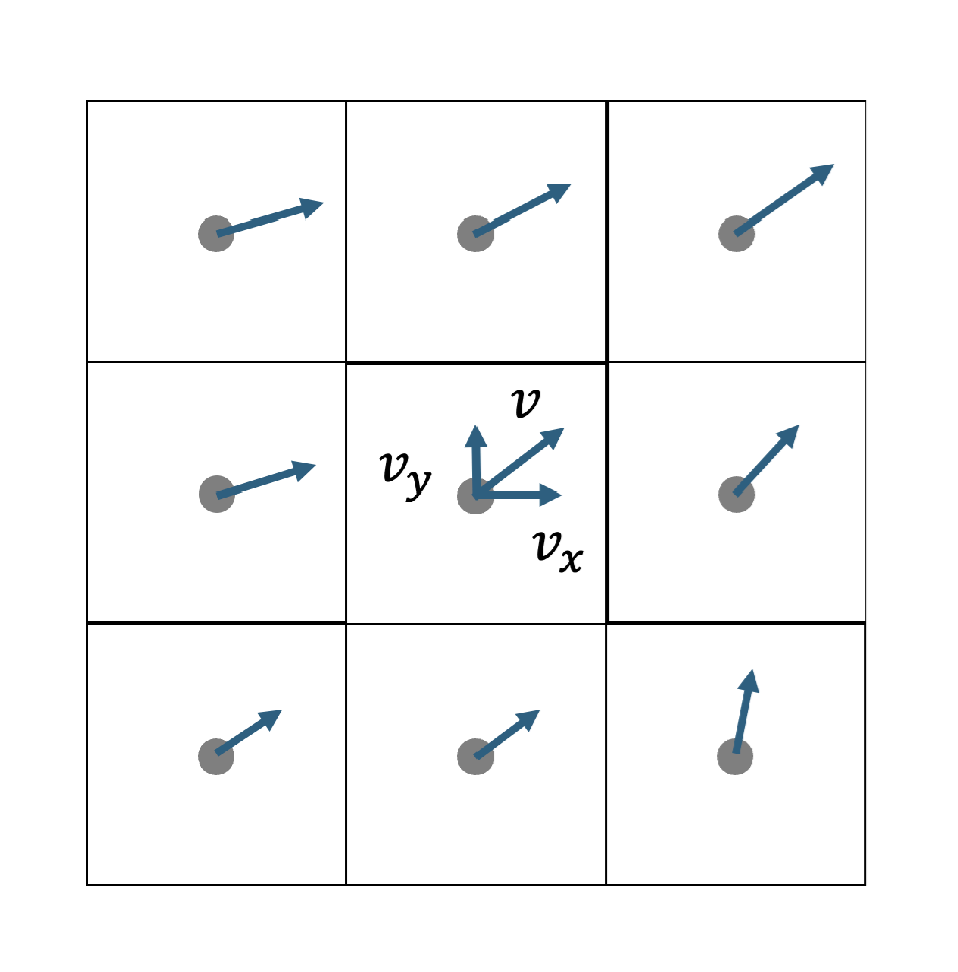
\includegraphics[width=5cm]{resources/collocated_grid_2.png}
	\end{subfigure}
	\hfill
	\begin{subfigure}[t]{0.45\textwidth}
		\centering
		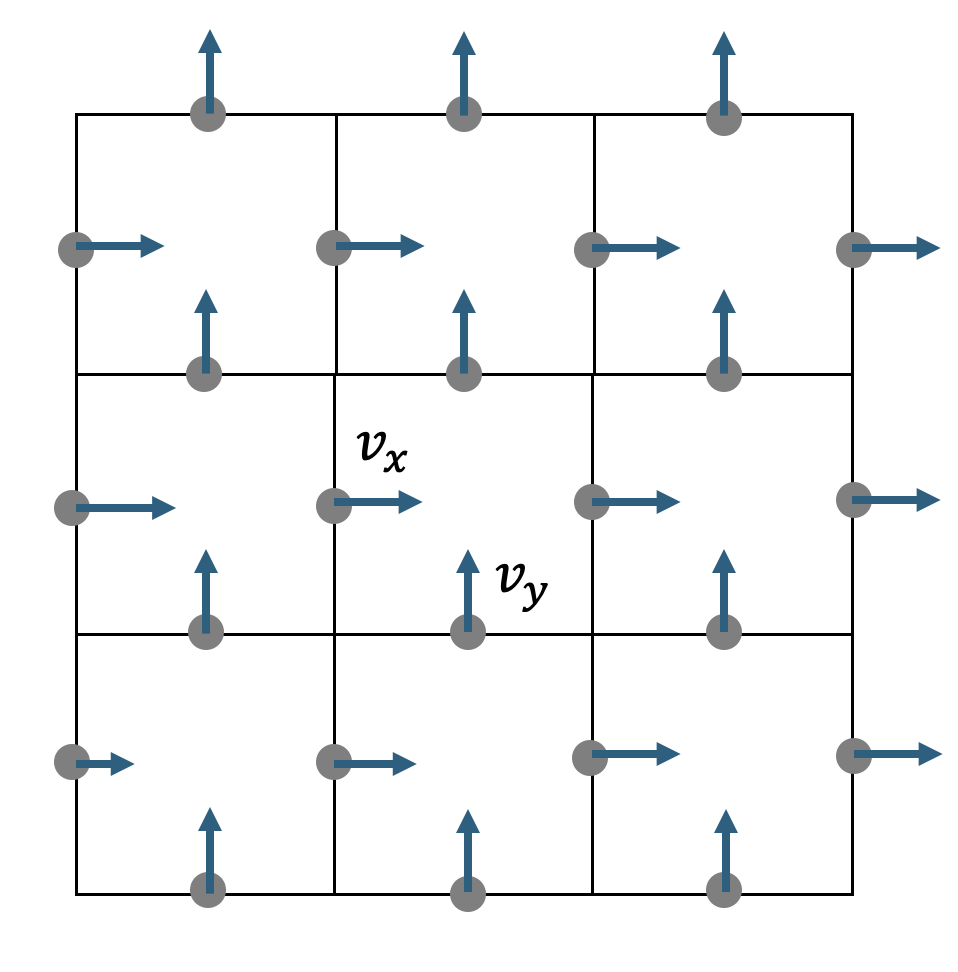
\includegraphics[width=5cm]{resources/staggered_grid_2.png}
	\end{subfigure}
	\caption{Computational grids}
\end{figure}

There are two different types of velocity vector fields we can use: collocated and staggered.
In the collocated grid all the variables are stored in the center of the cell,
whereas in the staggered grid the scalar variables are stored at the center but the velocity variable is stored at the cell face. 
Usually the use of a staggered grid is preferred, because it's easier to see how much fluid flows from one cell to another (\cite{tenminute}).
However, because Mike Ash and Jos Stam used a collocated grid in their works we decided to use the same grid for the sake of simplicity.

\subsection{Density Solver} \label{density}

First, let's look at the density solver. The density solver follows three steps:
adding forces, then applying diffusion and lastly moving the densities. 
If we look at the density equation in section \ref{math}, we see that the change in density in a single time step is influenced by three terms. 
The first term states that the density should follow the velocity field,
the second term represents the density's rate of diffusion
and the third term says that the density can increase due to external sources. 
The density solver will apply these terms in reverse order. 
So, as stated before, first the forces are added, then the diffusion is applied and finally the densities are moved.

\subsubsection{Adding forces}
The first step is adding forces from a source. In our case forces will be added if the user clicks on the screen.
If that happens we will simply add a constant amount of density to the intial density. So:
\[
\begin{array}{ll}
  \rho_{t+dt} = \rho_t + S \cdot dt
\end{array}
\]

\subsubsection{Diffusion} \label{diffusion}
The second step is diffusion.
Diffusion is the process where the fluid spreads from high density cells to low density cells.
The diffusion happens at a constant rate that we will call \textit{D}. 
Now we can simply calculate the diffusion rate \textit{a} by multiplying it with the time step:
\[
\begin{array}{ll}
  a = dt \cdot D
\end{array}
\]
If we take a look at a single cell, we'll see that it exchanges densities with its four neighbors (in 2D, the same applies for a 3D cell's six neighbors).
The total difference of the densities between the cell and its neighbors can be calculated by the following formula,
where $\rho_{x, y}$ is the current density of the cell at position $(x, y)$:
\[
\begin{array}{ll}
	\rho_{x+1, y} + \rho_{x-1, y} + \rho_{x, y+1} + \rho_{x, y-1} - 4 \cdot \rho_{x, y}
\end{array}
\]
By multiplying the difference in densities with the diffusion rate \textit{a} and adding it to the current density, we calculate new density of the cell. 
This can be seen in the following formula, where P$_{x, y}$ is equal to the density of cell at position $(x, y)$ after the time step:
\[
\begin{array}{ll}
	P_{x, y} = \rho_{x, y} + a \cdot (\rho_{x+1, y} + \rho_{x-1, y} + \rho_{x, y+1} + \rho_{x, y-1} - 4 \cdot \rho_{x, y})
\end{array}
\]
But here we run into a problem. If the diffusion rate is big enough, the density in a cell might end up becoming negative.
Imagine, for example, a situation were the diffusion rate is equal to 1,  the density of a cell is 1 and the densities of its neighbors are all 0. This means that the density of the cell will become -3.
This of course is not possible.
The solution to this problem is to find the density of the cell when being diffused backwards in time. Which results in the following equation:
\[
\begin{array}{ll}
	\rho_{x, y} = P_{x, y} + a \cdot (P_{x+1, y} + P_{x-1, y} + P_{x, y+1} + P_{x, y-1} - 4 \cdot P_{x, y})
\end{array}	
\]
To solve this system of linear equations for the unknowns P$_{x, y}$ the \href{https://en.wikipedia.org/wiki/Gauss–Seidel_method}{Gauss-Seidel method} is used.
This is an iterative method to solve a system of linear equations. In short, we apply the following formula an N amount of times for every cell in the grid:

\[
	\begin{array}{ll}
		P_{x, y} = \frac{\rho_{x, y} + a \cdot (P_{x+1, y} + P_{x-1, y} + P_{x, y+1} + P_{x, y-1})}{1+4a}
	\end{array}
\]

N is a constant that determines how many times the formula is applied. The higher N is, the more accurate the result will be. (\cite{josstam})

\subsubsection{Advection}

\begin{figure}[H]
	\centering
	\begin{subfigure}{0.3\textwidth}
		\centering
		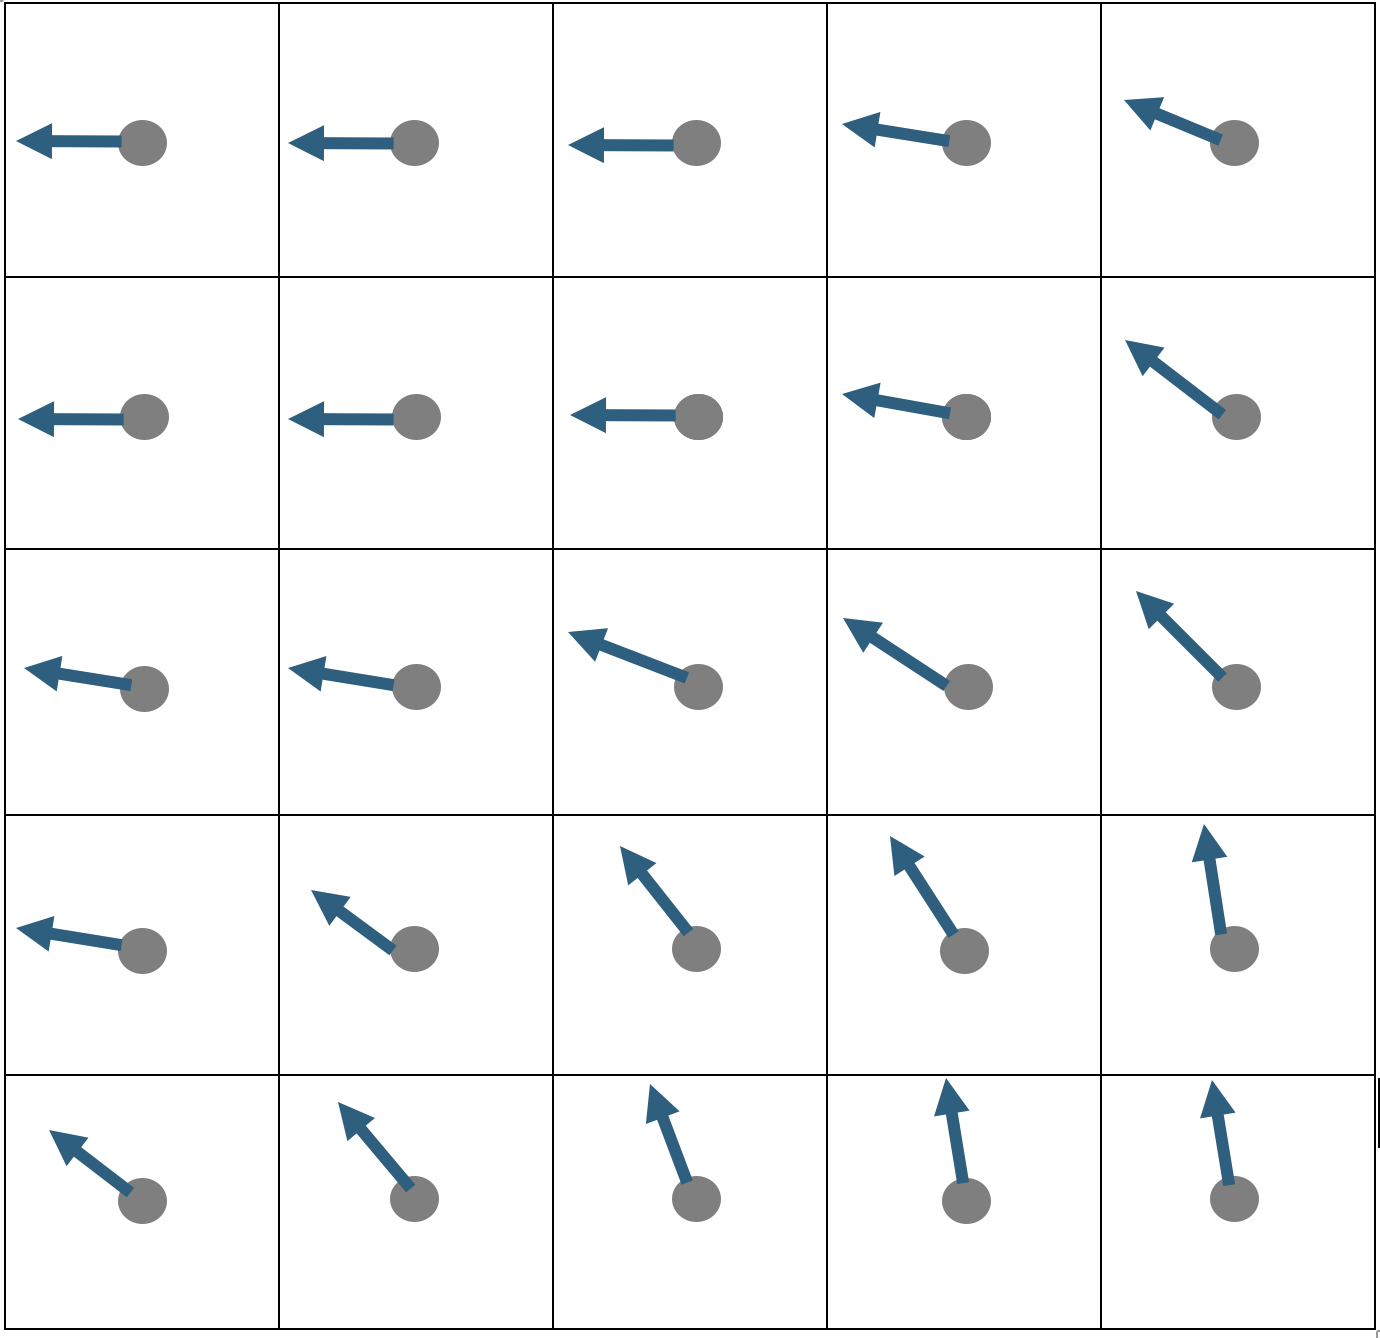
\includegraphics[width=4cm]{resources/advection1.png}
		\caption{Velocity vector field}
	\end{subfigure}
	\begin{subfigure}{0.3\textwidth}
		\centering
		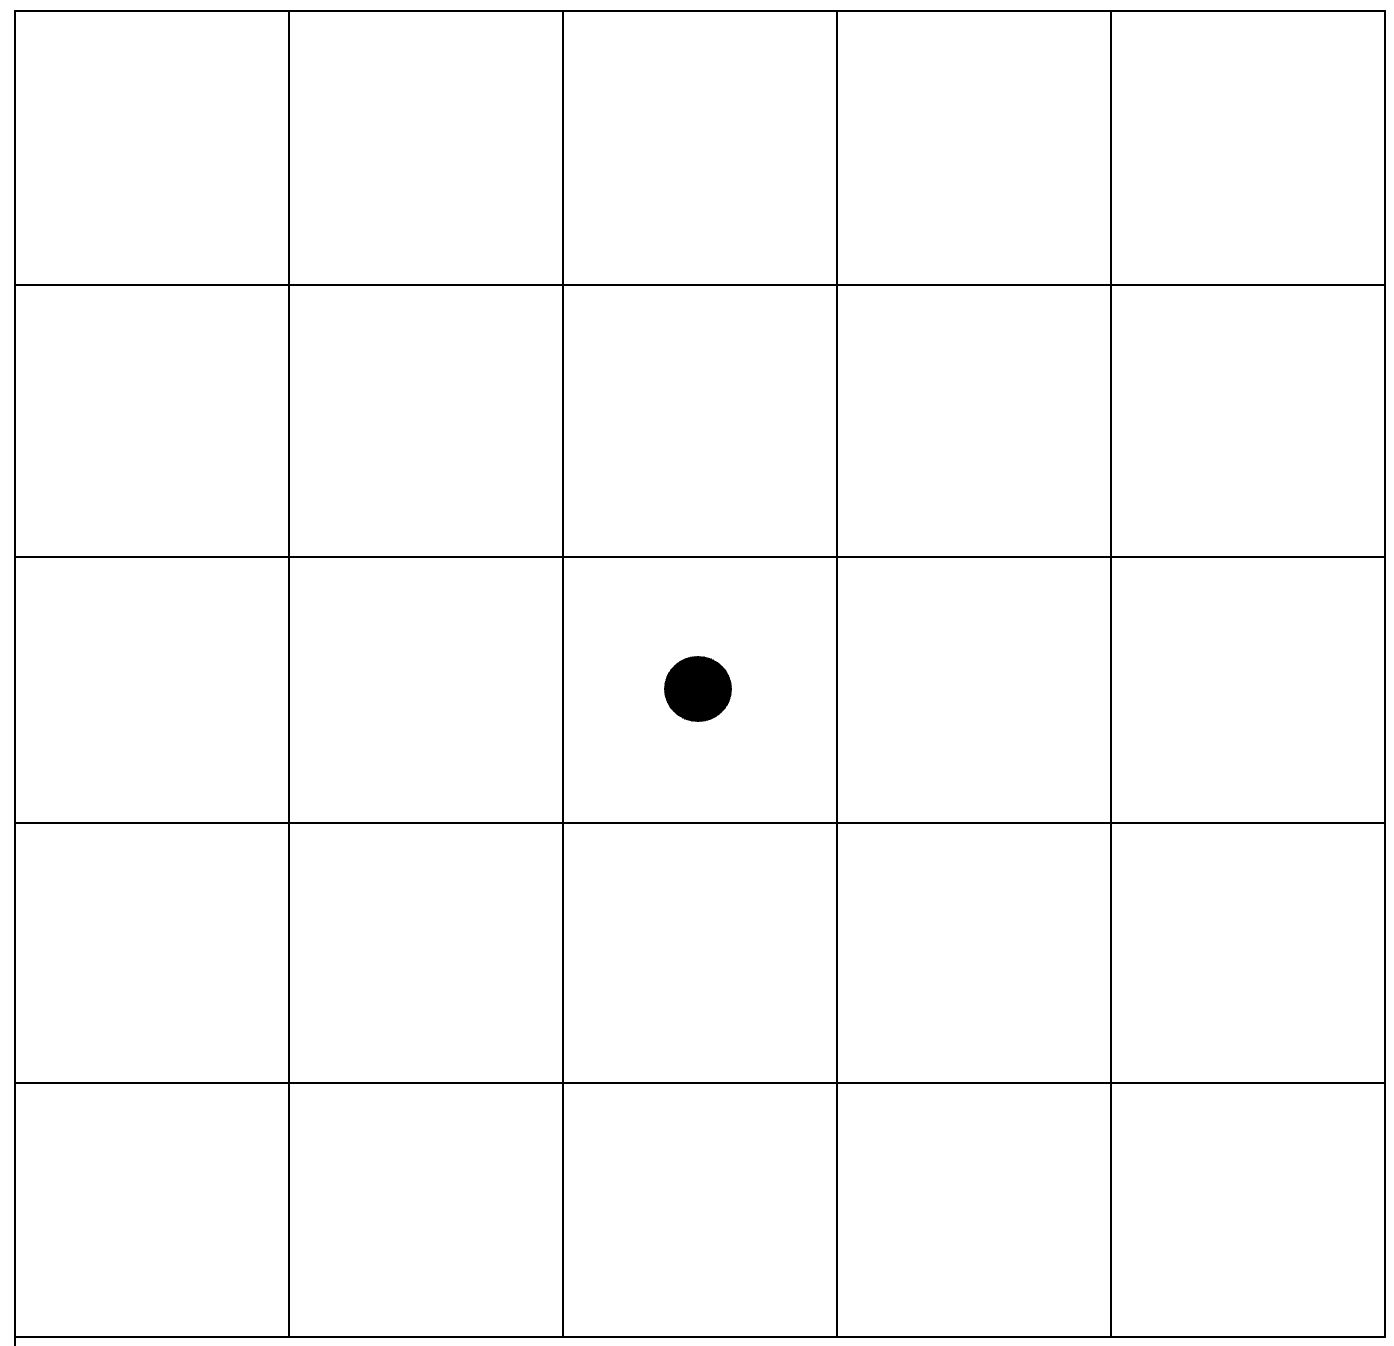
\includegraphics[width=4cm]{resources/advection2.png}
		\caption{A particle}
		\label{fig:aparticle}
	\end{subfigure}
	\begin{subfigure}{0.3\textwidth}
		\centering
		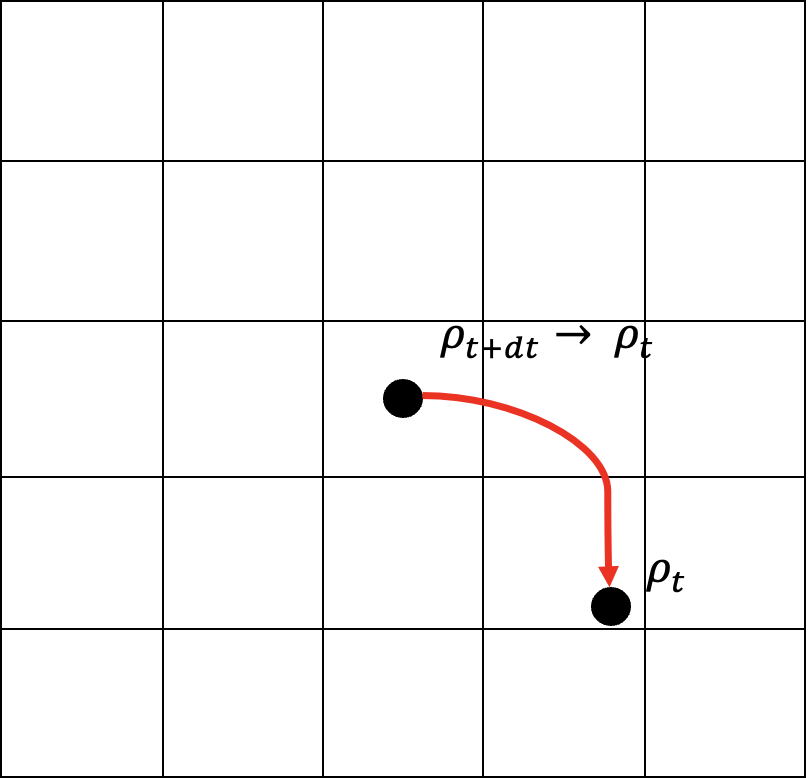
\includegraphics[width=4cm]{resources/advection3.png}
		\caption{Backtracing the particle}
		\label{fig:backtrace}
	\end{subfigure}
	\caption {Advection method}
	\label{fig:advection}
\end{figure}

The final step of the density solver is moving the densities following the velocity
field. Because you can't really move grid cells, we will use a technique where we
represent a density as a set of particles. This technique is called semi-lagrangian
advection. An obvious way to move the densities is to act like the center of a
cell is a particle and move it through the velocity field. But because we have
to convert the particles back to a grid, we will use a different method. We will
first look at the particles that end up at the center of a cell, as shown in
figure \ref{fig:aparticle}. Then we use the velocity of the cell to trace the particles
one time step back in time. This is shown in figure \ref{fig:backtrace}. Then we will
look at where the particles end up and calculate the weighted average of the
densities of the four closest cells from a particle and set this as the new density
of the current cell, also shown in figure \ref{fig:backtrace}. To do this we need to use
two different grids: one that contains all the density values from the previous
time step and on that contains the new density values. (\cite{josstam})
 
\subsection{Velocity Solver} \label{velocity}
Now we will look at the velocity solver. Just like with the density solver if we
look at the equations in section \ref{math} we see that the change in velocity
in a single time step is influenced by three factors. These are: the addition of
forces, viscous diffusion and self-advection. Because the velocity equation
looks so much like the density equation we can use the same steps that were shown
in section \ref{density} to solve it. The only difference is that the velocity
solver has an extra step called projection.

\subsubsection{Projection} \label{projectionstep}
This step ensures that mass is conserved. 
The law of conservation of mass is an important property of real-life fluids.
The projection step will be the last step that is executed because the previous
steps might not always conserve mass. To make the fluid mass conserving we will
use a mathematical concept called Hodge decomposition. Hodge composition states
that every vector field is the sum of a mass conserving field and a gradient field.
So all we have to do is compute a gradient field and subtract it from the velocity
field. The gradient field indicates the direction of steepest descent of a height function, as seen in figure \ref{fig:gradient_field}.
Computing this height field involves the solution of a linear system called a Poisson equation.
To solve this system we will we again use the Gauss-Seidel method that was also mentioned in section \ref{density} in the diffusion step (\cite{josstam}).

\begin{figure}[H]
	\centering
	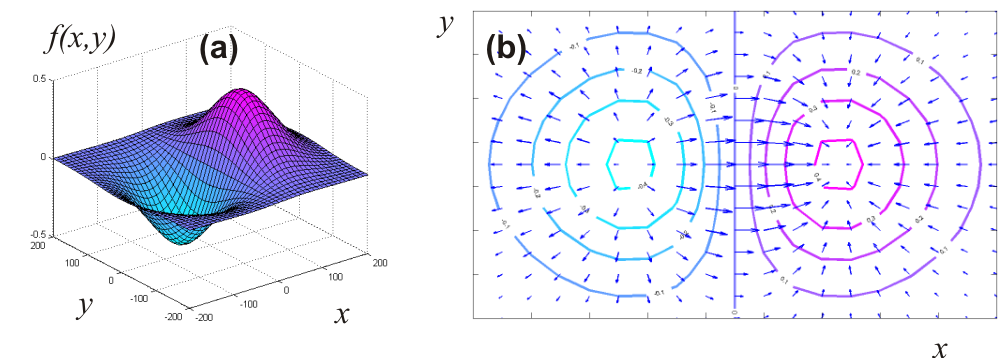
\includegraphics[width=15cm]{resources/gradient_field.png}
	\caption{Gradient field from (\cite{christophefinot})}
	\label{fig:gradient_field}
\end{figure}

\subsection{The Implementation} \label{implementation}
\subsubsection{Introduction to the code}
Our project is structured as follows:
\dirtree{%
	.1 paper.
	.2 neural\DTcomment{Contains ML engine}.
	.2 simulation/\DTcomment{Contains the physics simulation code}. 
	.3 include/\DTcomment{Our own engine headers}.
	.3 resources/\DTcomment{Resources like images, fonts, shaders}.
	.3 src/\DTcomment{Actual engine source}.
	.3 config.toml\DTcomment{Configuration file}.
	.3 Makefile.
}

This codebase is written in C++ and uses \href{https://www.raylib.com/}{raylib} again
because it's a really simple and powerful library that allows us to focus on the
simulation itself, as it provides a bunch of tools to easily render 3D graphics.
The reason this codebase is in C++ was initially because we never got the Eulerian
model to work in Go, likely due to a mistake of our own. Nevertheless we think C++
was the right choice, as it's more appropriate for the vector physics and low overhead
we need for the simulation.

The main fluid simulation object we use for the simulation is the \lstinline{Fluid} class.
The implementation is is available at \lstinline{/simulation/src/Fluid.cpp}.
The interface is as follows:

\begin{figure}[H]
	\centering
	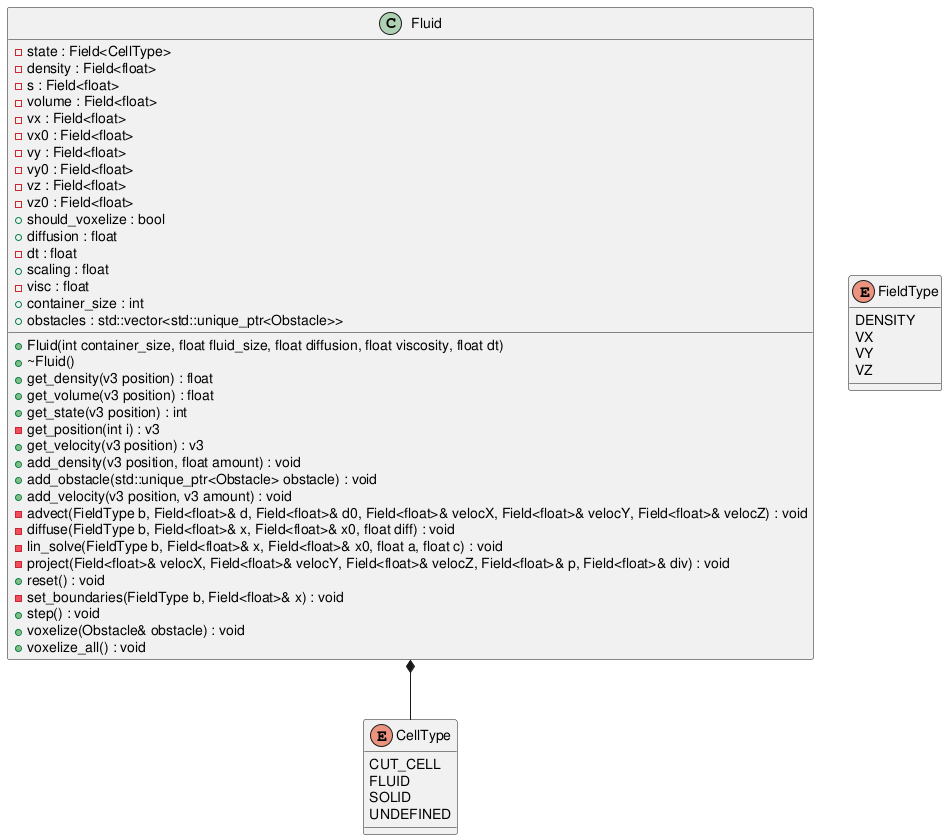
\includegraphics[width=\textwidth]{resources/Fluid.png}
	\caption{Fluid class diagram}
	\label{fig:interface}
\end{figure}

This class contains the vector fields for the container as well as all the
functions related to the physics simulation, including the advection, diffusion
and projection procedures. These functions are the core of the CFD and
this is the part that we borrowed from Mike Ash. After implementing the
interface of figure \ref{fig:interface} along with some graphical
rendering code, we were able to get a basic fluid simulation working. The
result is shown in figure \ref{fig:core}.

\begin{figure}[H]
    \centering
    \begin{subfigure}[t]{0.45\textwidth}
        \centering
        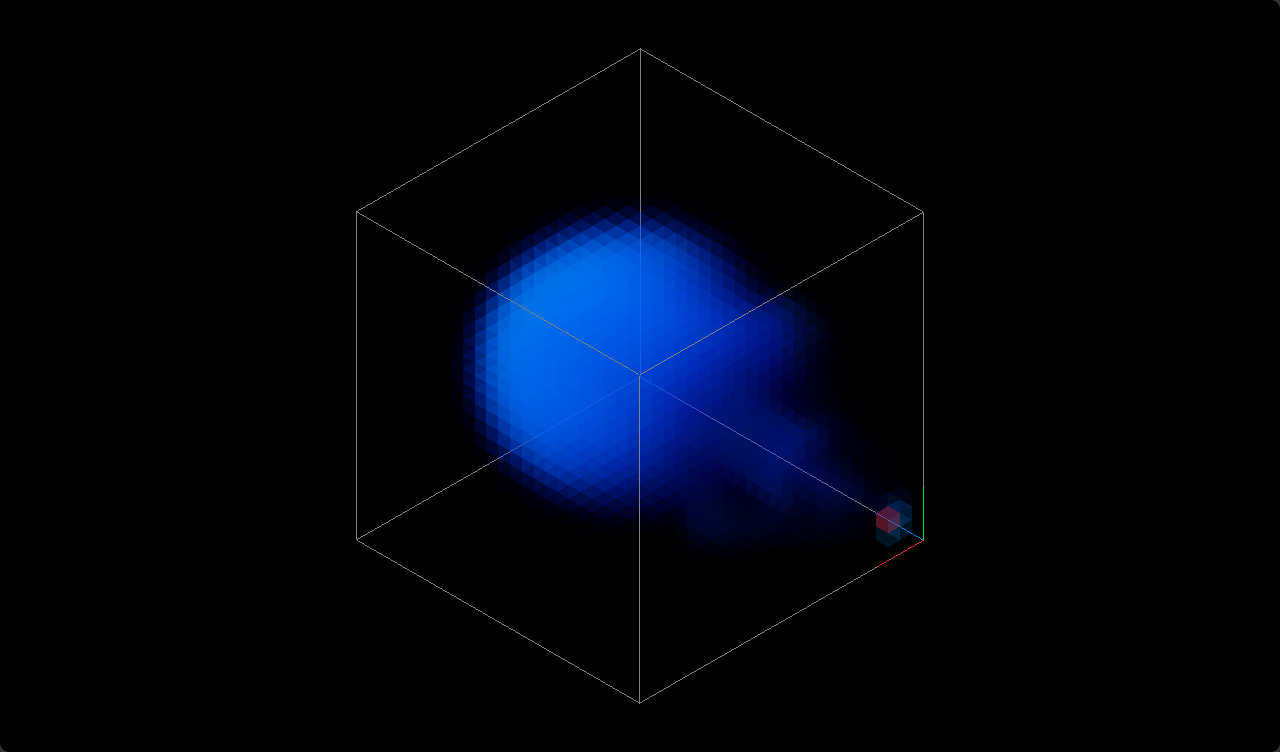
\includegraphics[height=1.65in]{resources/core1.png}
    \end{subfigure}
    \hfill
    \begin{subfigure}[t]{0.45\textwidth}
        \centering
        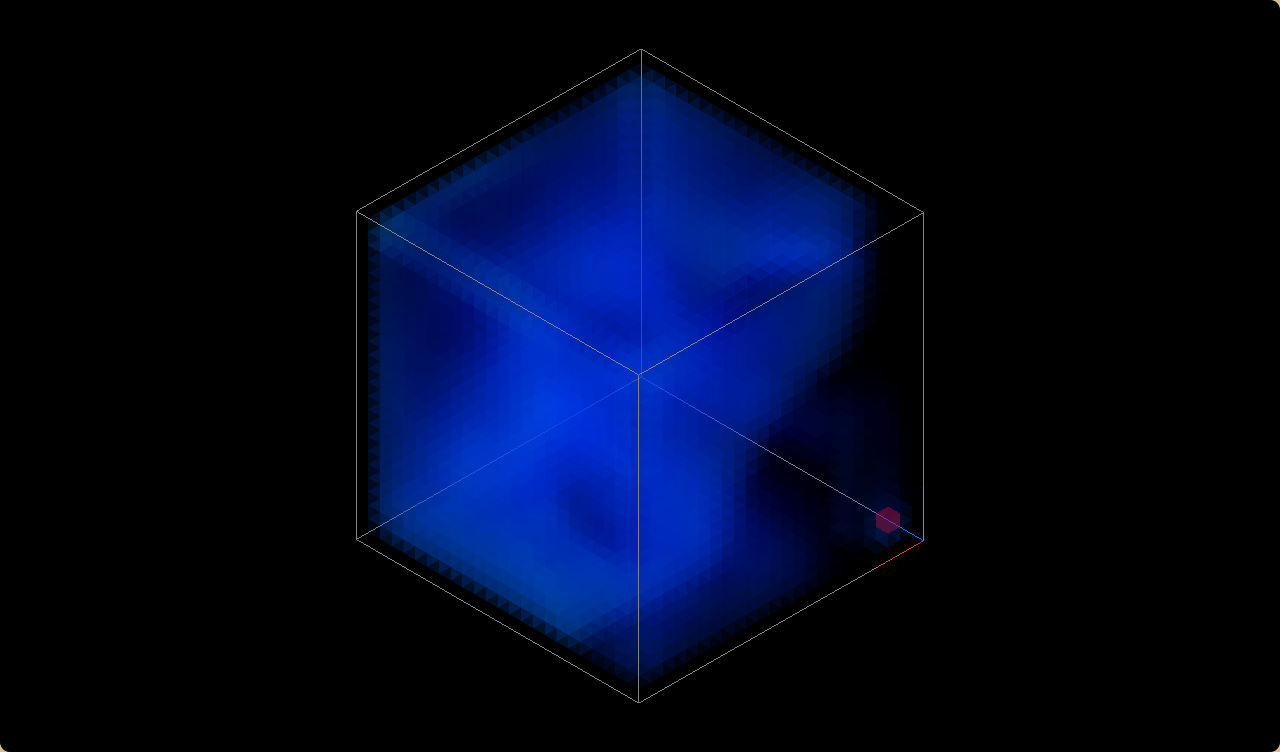
\includegraphics[height=1.65in]{resources/core2.png}
    \end{subfigure}
	\caption{Basic fluid simulation}
	\label{fig:core}
\end{figure}

\subsubsection{Voxelizing Geometry}
The next step is to implement geometry collision. The graphics library we're using,
Raylib, has a function to load geometry from object files. Loading in an arbitrary shape
like a torus is easy enough, but the real challenge lies in communicating to the
CFD that there's a torus in a given position and it behaving correspondingly.

First, the 3D object that Raylib loads has to be converted to a BVH (Bounding Volume
Hierarchy) object. This is a tree structure that contains the object's geometry in
a way that makes it easy to check if a point is inside the object. This format
is what FCL (\href{https://github.com/flexible-collision-library/fcl}{Flexible Collision Library})
uses to check for collisions. We are using FCL to easily process flexible
collisions between 3D objects.

The next step is to write a voxelization function. Voxelization takes a 3D
object's mesh data and iterates over the cells of the 3D
vector fields to see if the object occupies a cell or a part of a cell. FCL performs
collision detection between two 3D objects. In this case those two objects are
our obstacle (like a torus or a plane), and whichever cell is being iterated over.
If the cell that's being iterated over contains part of an object, we can pass
a corresponding condition to the CFD. This is done for every cell in the grid,
and the result is a 3D boolean array that represents the object. The source code
is at \lstinline{Fluid::voxelize}. Each obstacle is passed to this function, and
as a result we get a 3D boolean field saved at \lstinline{Fluid::state}.
\ref{fig:voxelmap} is a figure of the voxel map, with cells classified as solid highlighted in
blue. Note that the edges of the torus are also marked as solid despite their cells
obviously only being partial. This is because our implementation of the voxel mapping
using FCL isn't working as intended.

\begin{figure}[H]
    \centering
    \begin{subfigure}[t]{0.45\textwidth}
        \centering
        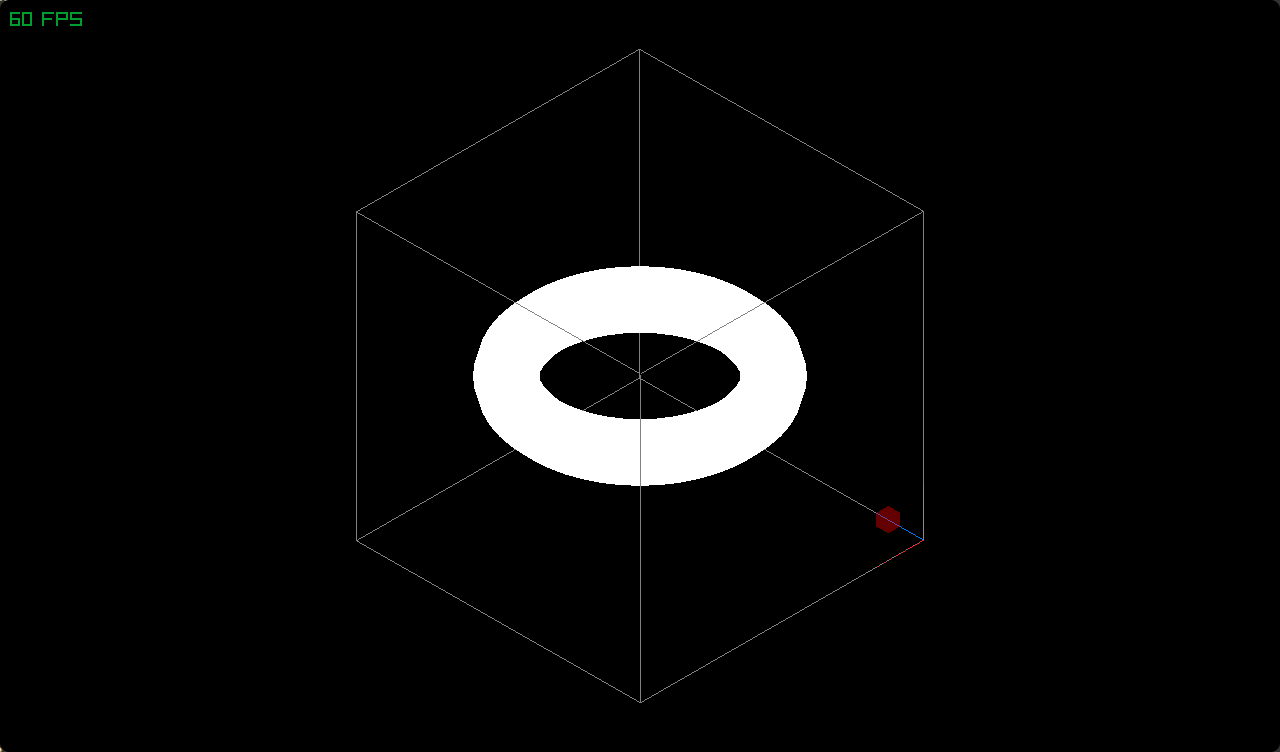
\includegraphics[height=1.65in]{resources/voxelize1.png}
		\caption{}
    \end{subfigure}
    \hfill
    \begin{subfigure}[t]{0.45\textwidth}
        \centering
        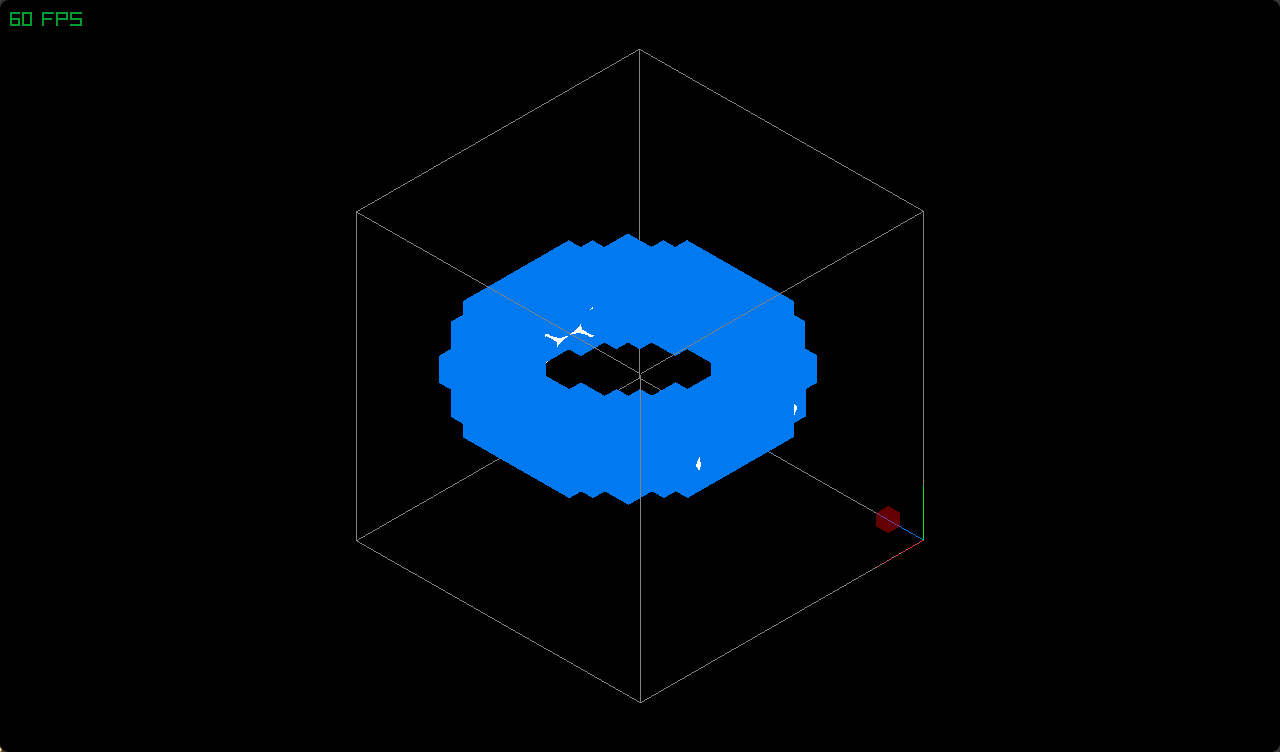
\includegraphics[height=1.65in]{resources/voxelize2.png}
		\caption{}
		\label{fig:voxelmap}
	\end{subfigure} 
    \caption{Voxel map}
\end{figure}

This is called the \href{https://www.sciencedirect.com/science/article/pii/S0307904X00000056}{Cut-Cell method} (\cite{cutcell}). The reason we even need this is because
the more obvious option is to set up the grid to be high resolution so each cell
is small enough to accurately approximate an arbitrarily complex object. The
reason this isn't viable is purely due to performance. This might be reasonable
with a supercomputer, but for our purposes we'd just like to optimize.

Another method would be to implement an AMR (Adaptive Mesh Refinement) system,
which would adapt the mesh's resolution based on what's in a given region (\cite{amr}). This would
generate a high resolution grid around an obstacle's bounds, and a low resolution
grid in any empty space. This is an interesting concept, but we would have to
rewrite some of the fluid math code to make the irregular grid work, and the Cut-Cell
method is more straightforward, so we stuck with that.

\subsubsection{Implementing obstacle collision}
According to the Cut-Cell method, each cell of the grid now has one of three states:
fluid, solid, or cut-cell.

\begin{minipage}[t]{0.65\textwidth}
	\begin{enumerate}
		\item{Fluid cells}
			\begin{itemize}
				\item{Cells that are fully inside a fluid region}
				\item{Normal Navier-Stokes equations apply}
			\end{itemize}
		\item{Solid cells}
			\begin{itemize}
				\item{Cells that are fully inside an obstacle}
				\item{Applies no-slip condition: velocity is zero}
			\end{itemize}
		\item{Cut-cells}
			\begin{itemize}
				\item{Cells partially inside an object}
				\item{Modify fluid calculations}
			\end{itemize}
	\end{enumerate}
\end{minipage}\hfill
\begin{minipage}[t]{0.3\textwidth}
	\vspace{10pt}
	\centering\raisebox{\dimexpr \topskip-\height}{%
	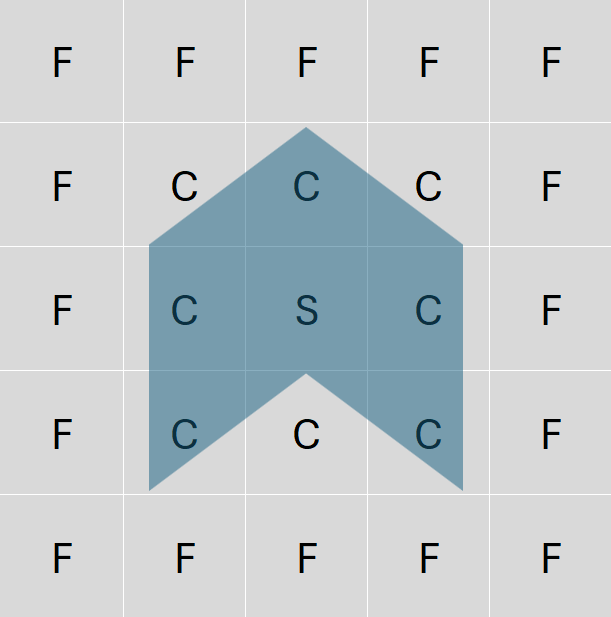
\includegraphics[width=\textwidth]{resources/voxeldiagram.png}}
	\captionof{figure}{Diagram of cell states}
	\label{fig:voxeldiagram}
\end{minipage}
\vspace{10pt}

We'd like to preface this by saying that our implementation of Cut-Cell obstacle
resolution is not completed or working, so some of the following is theoretical.
The idea is that when a cell is classified as a Cut-Cell, we create a new field to
track the amount of fluid that's inside the cell. For every cell, we calculate the
fractional fluid volume:

\[
	\begin{array}{ll}
		\text{Fractional fluid volume } \alpha = \frac{\text{volume of fluid in cell}}{\text{total cell volume}} \\
		\\
		\text{Fractional face area } \beta_d = \frac{\text{open d-face area}}{\text{total d-face area}} \text{ where d is one of $x$, $y$, or $z$}
	\end{array}
\]

The fractional fluid volume is the ratio of the volume of fluid in the cell to the
total volume of the cell, where a solid cell has a value of 0 and an empty cell has
a value of 1. The same goes for the fractional face area, which is the ratio of the
open face area to the total area of a given cell.

With this information we can modify the advection step of the CFD to account for
a cut-cell. We do this by scaling the advection by the fractional face area. Next
we also adjust the \hyperref[projectionstep]{projection step}. The projection step
is where we ensure that mass is conserved. We do this by scaling the pressure
field by the fractional fluid volume and fractional face area. The formula for pressure
given in section \ref{diffusion} is modified to:
\[
	\centering
	P_{x, y, z} = \frac{
		\frac{1}{\Delta t} \nabla \cdot u + \beta_x^+ P_{x+1, y, z} + \beta_x^- P_{x-1, y, z} + \beta_y^+ P_{x, y+1, z} + \beta_y^- P_{x, y-1, z} + \beta_z^+ P_{x, y, z+1} + \beta_z^- P_{x, y, z-1}
	}{
		\alpha (\beta_x^+ + \beta_x^- + \beta_y^- + \beta_z^+ + \beta_z^-)
	}
\]

The last step is to make sure to apply the correct boundaries to the fluid,
where any solid cells have a constant velocity of 0.

The reason we failed to implement this is twofold:
\begin{enumerate}
	\item{
			Incomplete voxelization process. Figure \ref{fig:voxelmap} is
			captured with a modified version of the program that only voxelizes
			to two states: solid and fluid, with no cut-cells. This is because we
			weren't capable of implementing the FCL collision detection correctly.
			We don't know what caused the issue, but unfortunately we didn't have
			time to debug it thoroughly.
		}
	\item{
			We'd forgotten to modify the projection step to account for cut-cells,
			which explains a bug we experienced, where the fluid would leak through
			the cut-cells.
		}
\end{enumerate}

Improving on these two points would have yielded better results.

\pagebreak
\section{Machine Learning Theory}
The second part of our project was to use machine learning to optimize the shape
of the airplane's body. The idea was to use a genetic algorithm to evolve the
shape of the airplane's body to maximize performance. Once again since we didn't
have a working fluid simulation we never got around to actually writing this part.

That being said here's the outline of how ML (Machine Learning) works: we grab
a basic airplane model, and we generate a population of airplane models. We
simulate the airflow around each airplane model, and we use the results to calculate
a fitness score for each airplane model. We then use a genetic algorithm to evolve
the airplane models to maximize the fitness score. We repeat this process until
we have a model that approaches a maximum fitness score.

The plan was to write a Python script that utilizes the NEAT algorithm to generate
the populations. NEAT is a genetic algorithm, which has a Python library that
the user can implement in their scripts.

There's two big parts to this: the first is the fitness function, which is the
function that takes the results of the fluid simulation and calculates a score
for the airplane model. This is discussed in section \ref{fitness}.
section \ref{genalg} discusses the genetic algorithm, which is the portion that tweaks
the vertex data of each airplane model to try to improve the fitness score.

\subsection{Fitness Calculation} \label{fitness}
The fitness function is the function on the CFD-side that measures how good a
given polygon is at flying. The metric for this is the lift-to-drag ratio, which
is a measure of how much lift the airplane generates compared to how much drag
it generates. The lift-to-drag ratio is a good measure of how efficient an airplane
is at flying and it's a good way to quantify aerodynamic performance. We want the
lift-to-drag ratio to be as high as possible. To achieve that we need to try
to maximize lift and minimize drag.

The lift force $L$ primarily exists because of the pressure difference between
the top and the bottom of a wing. The integrals for the lift and drag forces are
listed below (\cite{liftdrag}).
\[
	\begin{aligned}
		& \text{where:} \\
		& \text{shear stress } \tau \\
		& \text{pressure } P \\
		& \text{surface of the wing } A \\
		& F_L = -\int_A (P \sin \theta + \tau_w \cos \theta) dA \\
		& F_D = \int_A (-P \cos \theta + \tau_w \sin \theta) dA
	\end{aligned}
\]


We can discreetly approximate these integrals by summing the pressure difference
over the surface of the wing:
\[
	\begin{array}{l}
		\text{where $i$ is a triangle of the wing:} \\
		F_D = \sum\limits_i (P_i \cos \theta_i + \tau_{w_i} \sin \theta_i) \cdot A_i \\
		F_L = \sum\limits_i (-P_i \sin \theta_i + \tau_{w_i} \cos \theta_i) \cdot A_i
	\end{array}
\]

Now that we have a formula for the lift and drag, we can calculate the lift-to-drag
ratio by dividing the lift by the drag. This is the fitness score that we will
use to evaluate the airplane models.

\subsection{Genetic Algorithm} \label{genalg}
This is the final part of the project, where the working fluid simulation and a
correct fitness function both converge. Since we never got around to implementing
the whole Machine Learning part of the project, we can't really give any specifics
on how our genetic algorithm should work. Knowing how to calculate the fitness
score is a good start, but the actual population generation and mutation requires
some trial and error with the different parameters of the genetic algorithm.
What we can talk about is how we would mutate the airplane models. This is the
part where the genetic algorithm tweaks the airplane models to try to improve
the fitness score.

The idea is to take the vertex data of the airplane model and apply some random
mutations to it. This could be anything from changing the position of a vertex
to adding a new vertex. The idea is to make small changes to the airplane model
and see if the fitness score improves. If it does, we keep the change, if it
doesn't we discard it. This is the basic idea behind the genetic algorithm.

% Conclusion
\pagebreak
\section{Conclusion}
In our paper we tried to answer the question: What is the most optimal shape for an airplane to maximize its aerodynamic performance?
This lead to the following subquestions:  \\

\textbf{SQ1:} How does a basic CFD simulation work?

\textbf{SQ2:} How is a CFD model implemented?

\textbf{SQ3:} How do obstacles work in a CFD?

\textbf{SQ4:} How is the performance of an airplane calculated?

\textbf{SQ5:} How can machine learning be used to optimize an airplane's shape? \\

To answer the questions 1 and 2 we looked the different methods that can be used to simulate fluid dynamics and the math behind them.
Most CFD models are based on the Navier-Stokes equations. These equations describe the flow of fluid. 
The two main methods for implementing these equations are: the Lagrangian method and the Eulerian method. 
We first tried implementing a Lagrangian fluid simulation, in this model fluid is represented by particles.
While trying to create this model we ran into some issues and decided to switch to a Eulerian fluid simulation.
In a Eulerian fluid simulation the fluid is represented by a grid of cells, where each cell has a velocity and density value.
The density solver in our simulation used three steps: adding forces, applying diffusion and moving the densities.
The velocity solver used the same steps as the density solver but with an extra step called projection.
We decided to use C++ and the Raylib library to implement the fluid simulation. 

To answer question 3 we created a cell state map that classified each cell as fluid or solid, but failed to recognize cut-cells.
We set up a pressure formula to account for cut-cells.

To answer the question 4 researched the lift-drag ratio, which is a measure of how efficient an airplane is at flying.
We set up an approximation for the lift and drag forces.

To find the answer to the last question we wanted to use a genetic algorithm to evolve the shape of an airplane's wing 
and analyze the performance of the different shapes in the fluid simulation. 

In the end we were not able to complete the research as we had hoped. We were able to create a basic fluid simulation, 
but we were not able to fully implement the obstacle collision detection. Because the CFD model was not working as intended, 
we were also not able to implement the machine learning part of the research.

% Results
\pagebreak
\section{Discussion: Challenges, Failures \& Future Work}
Due to the issues with the voxelization process and the object collisions, we
weren't actually able to complete the model we wanted. We have a working fluid
simulation, but most of the work we did on the obstacles was more theoretical
than any tangible working prototype. Here's an outline of what went wrong:

\subsection{Grid Collision}
\begin{itemize}
	\item{\textbf{Issue}: air bleeds through obstacles}
	\item{\textbf{Causes}:}
		\begin{itemize}
			\item{Cut-cell method not fully implemented}
			\item{Failure in voxelization process}
		\end{itemize}
	\item{
			\textbf{Solution}: it took a lot of trial and error, but no solution
			was found. We have some hypotheses, but we don't have any time to test,
			so it's possible that some of the solutions defined in this paper don't
			work in practice.
		}
	\item{\textbf{Result}: a dead end. Most of our project relied on this section working.}
\end{itemize}

\subsection{Performance}
Despite being written in 2006, Mike Ash's isn't the fastest, even with today's
hardware. The fluid simulation runs quite reasonably at a resolution, of say
$32\times32\times32$, but bumping up the grid size yields worse and worse results.
At that grid resolution of $32^3$, we see about 20 FPS on my laptop. This isn't
abysmal by any means, but $32^3$ really isn't very high either. So we profiled
the program to see what was the slowest.

\begin{figure}[H]
	\centering
	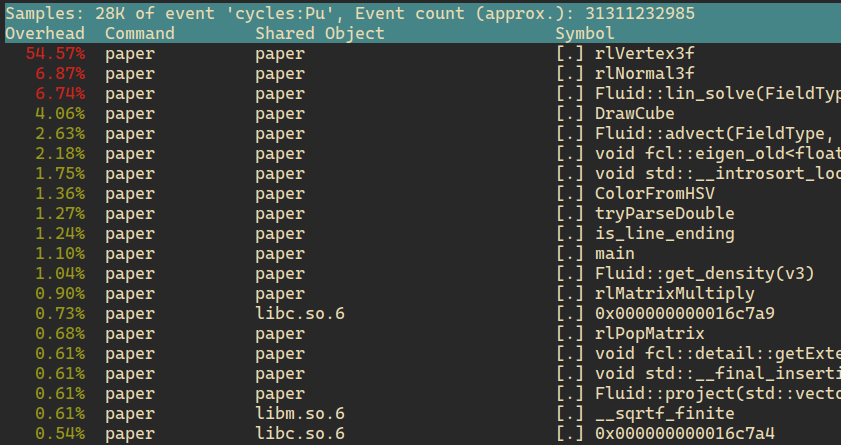
\includegraphics[width=\textwidth]{resources/profile.png}
	\caption{Profile of the fluid simulation program}
\end{figure}

Some of the steps involved in the Eulerian fluid simulation require iterating
over every cell in the grid, and performing some arithmetic operations on that cell.
Both the advection and projection steps require this, and the advection step
alone runs four times every step. That's about $32^3 \times 4 = 131\,072$ iterations
every step, just for the advection. This is understating the amount of arithmetic
operations that are executed, but it already gives an idea of the scale of the
problem.

We haven't optimized the code that much, but the most important thing we did was
parallelize the these large iterations. Anytime we have any meaningful iteration
over the grid, we use \href{www.openmp.org}{OpenMP} to parallelize it. This was
a very quick and simple way to get a performance boost, and it works quite well.
Still, there's some room for improvement.

We didn't actually go any further but we have some ideas for speed boosts. These
are speed boosts and not real algorithmic optimizations because for that we'd have
to really look into the Navier-Stokes equations and speed up Jos Stam's algorithms,
but that's beyond the scope of what we'd want to do. Rather we're thinking that
while we parallelized the long for loops, the code still isn't really asynchronous.
OpenMP is a great tool for parallelization, which is what we're using it for,
but we could go one step further and refactor our code to be truly asynchronous,
and assign a thread to each task, for example.

Another factor is that while the client-side rendering is hardware accelerated,
the actual fluid simulation all runs on the CPU. This is quite the bottleneck,
as the CPU architecture isn't really designed for this kind of large scale
parallel work for high resolution grids. Brute-forcing this would require a lot
of compute cores, which CPUs don't have (modern CPUs have between 4 and 16 cores
in the consumer market). The most obvious solution is to transfer the load to
a dedicated GPU, which we can utilize to perform all these arithmetic operations
for us and would yield a massive improvement. Migrating the CFD code to a compute
shader or an \href{https://en.wikipedia.org/wiki/OpenCL}{OpenCL kernel} would
be a great way to speed up the simulation. This is something that would be very
fun to explore in the future, but once again it's beyond the scope (and time limit)
of our project.

\subsection{Future Work}
Considering the amount of ideas that have failed, there's a lot of room for
improvement. In the future, there's a very specific order of operations that
we'd like to follow to get the project to a working state.
\begin{enumerate}
	\item{Fix the voxelization process}
	\item{Implement a working Cut-Cell (or AMR) method}
	\item{Possible further optimize the fluid simulation}
	\item{Finish with a working genetic algorithm}
\end{enumerate}
Once that's all completed, we'd truly have answered all the questions we set out
to answer in this paper.

\pagebreak
\section{Eigen-werk verklaring}
Ondergetekende …………………………………………………… verklaart:

\begin{itemize}
	\item{dat dit PWS eigen werk is}
	\item{dat alles wat overgenomen is uit enige bron voorzien is van een correcte bronvermelding}
\end{itemize}

Heemstede, [datum]…………………………………………………………2025 \\

Handtekening: \\ \\

Ondergetekende …………………………………………………… verklaart:

\begin{itemize}
	\item{dat dit PWS eigen werk is}
	\item{dat alles wat overgenomen is uit enige bron voorzien is van een correcte bronvermelding}
\end{itemize}

Heemstede, [datum]…………………………………………………………2025 \\

Handtekening: \\ \\

% Reference
\pagebreak
\section{Bibliography}
\nocite{*}
\printbibliography

\end{document}
